\chapter*{Frequency response of RME FIREFACE UCX}
A test was made to get a view of the frequency response of the RME FIREFACE ucx. The RME FIREFACE ucx is used for all measurement in this project, and therefore the frequency response is of interest. To measure the frequency response, the function from \autoref{appendix:transfer_function} is used.

\section*{Materials and setup}
To measure the frequency response of the RME FIREFACE UCX, the following materials are used:
\begin{itemize}
\item RME FIREFACE ucx (Soundcard)
\item MATLAB 2017b (PC - Software)
\item IRmeas_fft (software) \autoref{appendix:transfer_function}
\item jack to jack cable
\end{itemize}

\begin{figure}[H]
\centering
\begin{picture}(0,0)%
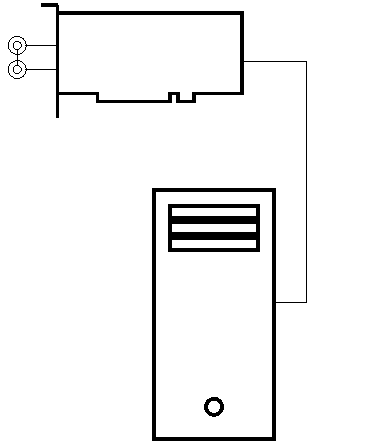
\includegraphics{rme_transfer_function.pdf}%
\end{picture}%
\setlength{\unitlength}{2818sp}%
%
\begingroup\makeatletter\ifx\SetFigFont\undefined%
\gdef\SetFigFont#1#2#3#4#5{%
  \reset@font\fontsize{#1}{#2pt}%
  \fontfamily{#3}\fontseries{#4}\fontshape{#5}%
  \selectfont}%
\fi\endgroup%
\begin{picture}(4090,4926)(8176,-7474)
\put(8191,-3661){Out}%
\put(9271,-3211){Sound Card}%
\put(9971,-6361){Computer}%
\put(11836,-4696){USB}%
\put(8281,-2806){In}%
\end{picture}%
\caption{Setup for measuring transfer function}
		\label{fig:appendix:rme_response}
\end{figure}

\section*{Test procedure}


\begin{enumerate}
\item The materials are set up as in \autoref{fig:appendix:test}.
\item The cable is connected between input 1 and output 1
\item The input gain at input 1 is set to \SI{20}{\decibel}
\item The output playgain is set to \SI{-18}{\decibel}
\item The input and output channel is specified in the MATLAB function "SynchronizedPlaybackAcquirer" 
\item IRmeas_fft (software) \autoref{appendix:transfer_function} is preformed
\item The transfer function is plotted from \SI{20}{\hertz} to \SI{20}{\kilo\hertz}
\end{enumerate}

\section*{Results}



On \autoref{fig:appendix:rme_response_result} it is seen that the soundcard only have a non linearity of \SI{0.26}{\decibel} from \SI{20}{\hertz} to \SI{20}{\kilo\hertz} between output data and input data. 

\begin{figure}[H]
	\centering
	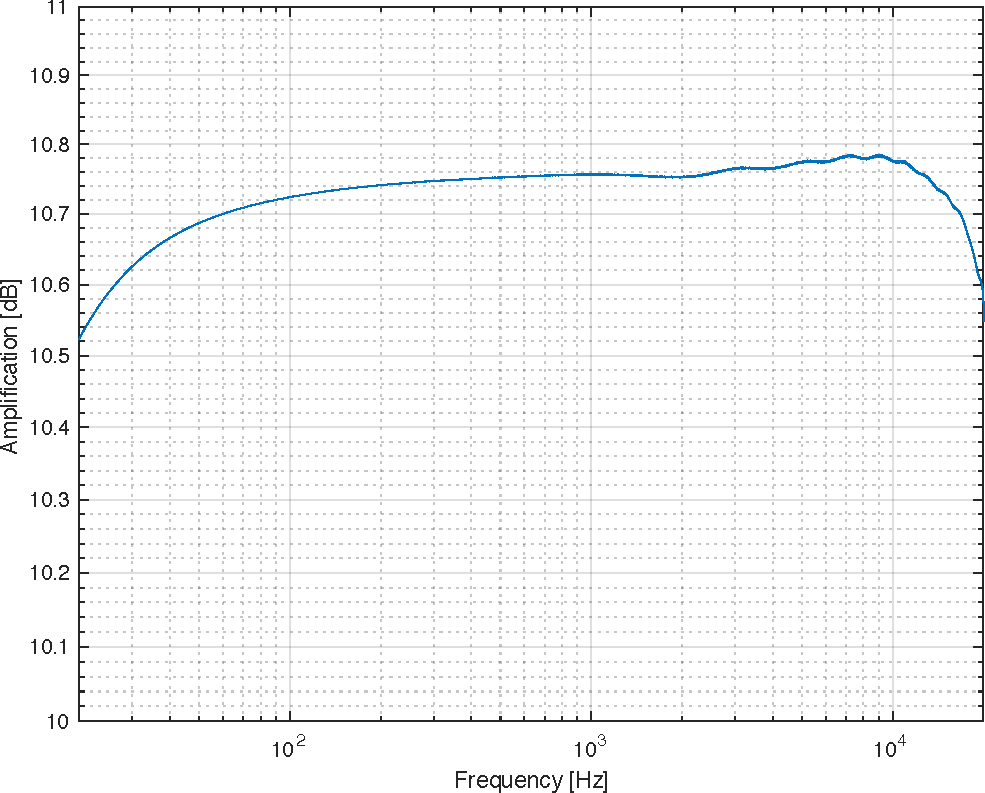
\includegraphics[width=1\textwidth]{RME_FIREFACE_UCX_tf.pdf}
	\caption{The frequency response of the RME FIREFACE UCX with input sensitivity at 20}
		\label{fig:appendix:rme_response_result}
\end{figure}

\section*{Conclusion}
It can be concluded that en RME_FIREFACE_UCX have a non linearity of \SI{0.26}{\decibel} when the input gain is at \SI{20}{\decibel} and the output playgain is at \SI{-18}{\decibel}


